\documentclass[../main.tex]{subfiles}

\graphicspath{{../images/}}

\begin{document}
\pagestyle{fancy}
\lhead{Homework 9}
\chead{Junseo Shin}
\rhead{PHYS 421}

%  HW 5: 5.14, 5.18, 5.26, 5.32, 5.36, 5.39
\begin{center}
    \section*{Homework 9}
    % add to toc
    \addcontentsline{toc}{section}{Homework9}
\end{center}

\paragraph{5.14} For a steady current $I$ flowing down a long cylindrical wire of radius $a$ the magnetic field inside and out the wire
\begin{itemize}
    \item [(a)] Given a uniform surface current
    \begin{align*}
        \oint B \cdot \dd{\vb l} = \mu_0 I_\text{enc} \implies B(2\pi s) = \mu_0 I \pi 
    \end{align*}
    where $s$ is the distance from the axis of the wire. Thus
    \begin{align*}
        \boxed{
            B = \frac{\mu_0 I}{2s} \quad s > a, \qand B = 0 \quad s < a
        }
    \end{align*}
    which is points in the $\vu*\phi$ direction.
    \item [(b)] For $\vb J \propto s$
    \begin{align*}
        J = ks \implies I = \int \vb J \cdot \dd{\vb a} = \int_0^a (ks) 2\pi s \dd{s}  = \frac{2\pi k a^3}{3}
    \end{align*}
    So the constant $k$ is
    \begin{align*}
        k = \frac{3I}{2\pi a^3}
    \end{align*}
    Outside the wire $I_\text{enc} = I$ so
    \begin{align*}
        \boxed{
            \vb{B} = \frac{\mu_0 I_\text{enc}}{2\pi s} \vu*\phi =  \frac{\mu_0 I}{2\pi s} \vu*\phi \quad s > a
        }
    \end{align*}
    But for $s < a$ the current only a fraction of the current is enclosed:
    \begin{align*}
        I_\text{enc} = \int_0^s ks' (2\pi s') \dd{s'} = \frac{2\pi k s^3}{3} = \frac{2\pi s^3}{3} \qt(\frac{3I}{2\pi a^3}) = I \frac{s^3}{a^3}
    \end{align*}
    Therefore
    \begin{align*}
        \boxed{
            \vb B = \frac{\mu_0 I}{2\pi s} \qt(\frac{s^3}{a^3}) \vu*\phi = \frac{\mu_0 I s^2}{2\pi a^3} \vu*\phi \quad s < a
        }
    \end{align*}
\end{itemize}

\newpage
\paragraph{5.18} A parallel plate capacitor with uniform surface charge $\pm \sigma$ moves at constant
speed $v$.
\begin{itemize}
    \item [(a)] Between the plates, the magnetic field is (using a rectangular Amperian loop perpendicular to the moving plate from Example 5.8)
    \begin{align*}
        \oint \vb B \cdot \dd{\vb l} = \mu_0 I_\text{enc} \implies B(2l) = \mu_0 K l
    \end{align*}
    so at each region of a single plate
    \begin{align*}
        B = \pm \frac{\mu_0 K}{2} = \pm \frac{\mu_0 \sigma v}{2}
    \end{align*}
    Above and below the plate, the magnetic field is zero
    \begin{align*}
        \boxed{
            B = 0 \qqtext{above and below the plate}
        }
    \end{align*}
    and between the plates
    \begin{align*}
        \boxed{
            B = \mu_0 K = \mu_0 \sigma v \qqtext{between the plates}
        }
    \end{align*}
    \item [(b)] The magnetic force per unit area on the upper plate is
    \begin{align*}
        \frac{F_\text{upper}}{A} &= \frac{1}{A} \int K \cross B \dd{A} \\
        &= K \cross B \\
        &= (\sigma v) \cross \frac{\mu_0 \sigma v}{2} \\
        &= \boxed{
            \frac{\mu_0 \sigma^2 v^2}{2}
        }
    \end{align*}
    \item [(c)] The speed required to balance the electrical force: From electrostatics the force on the upper plate is
    \begin{align*}
        F = \sigma E = \sigma \frac{\sigma}{2\epsilon_0} = \frac{\sigma^2}{2\epsilon_0}
    \end{align*}
    so for the forces to balance
    \begin{align*}
        \frac{\mu_0 \sigma^2 v^2}{2} = \frac{\sigma^2}{2\epsilon_0} \implies v = \frac{1}{\sqrt{\mu_0 \epsilon_0}}
    \end{align*}
    where the values are related to the speed of light $c$ by \href{https://en.wikipedia.org/wiki/Vacuum_permittivity#Value}{(From Wikipedia)}
    \begin{align*}
        \epsilon_0 \mu_0 = \frac{1}{c^2} \implies v = c
    \end{align*}
    So the force will balance at the speed of light $c$.
\end{itemize}

\newpage
\paragraph{5.26} What current density would produce the vector potential $A = k \vu*\phi$ in cylindrical coordinates?
Finding $\vb B \to \vb J$: 
\begin{align*}
    \vb B = \curl A =  \frac{1}{s}\begin{vmatrix}
         \vu*s & s \vu*\phi & \vu*z \\
        \pdv{s} & \pdv{\phi} & \pdv{z} \\
        0 & s(k) & 0
    \end{vmatrix}
    = \frac{1}{s} \pdv{s}(sk) \vu z = \frac{k}{s} \vu*z
\end{align*}
So using Amp\`ere's Law
\begin{align*}
    \vb J = \frac{1}{\mu_0} (\curl \vb B) = \frac{1}{\mu_0 s} \begin{vmatrix}
        \vu*s & s \vu*\phi & \vu*z \\
        \pdv{s} & \pdv{\phi} & \pdv{z} \\
        0 & 0 & k/s
    \end{vmatrix}
    = -\frac{1}{\mu_0 s} s \qt(\pdv{z} \frac{k}{s}) \vu*\phi = \boxed{ \frac{k}{\mu_0 s^2} \vu*\phi }
\end{align*}

\newpage
\paragraph{5.32} To find the magnetic field inside a solid sphere of
uniform charge density $\rho$, radius $R$, and angular velocity $\omega$:

From Example 5.11 we just change $\sigma \to \rho$ so
\begin{align*}
    \vb A (r, \theta, \phi) = \begin{cases}
        \frac{1}{3} \mu_0 R' \rho \omega r \sin\theta \vu \phi & \text{Inside sphere} \\
        \frac{1}{3r^2} \mu_0 R'^4 \rho\omega \sin\theta \vu \phi & \text{Outside sphere}
    \end{cases}
\end{align*}
where we integrate $R'$ from $0 \to r$ to find the potential $A_{\phi_\text{out}}$ and
$r \to R$ to find $A_{\phi_\text{in}}$: The potential is then the sum of the two
\begin{align*}
    \vb A &= \frac{1}{3} \vu*\phi \mu_0 \rho \omega r \sin\theta \int_r^R R' \dd{R'} 
    + \frac{1}{3r^2} \mu_0 \rho \omega \sin\theta \int_0^r R'^4 \dd{R'} \\
    &= \frac{1}{3} \mu_0 \rho \omega \sin\theta \qt[
        \frac{1}{2} (R^2 - r^2) + \frac{1}{r^3} \frac{r^5}{5}
    ] \vu*\phi \\
    &= \mu_0 \rho \omega r \sin\theta \qt[
        \frac{R^2}{6} - \frac{r^2}{6} + \frac{r^2}{15}
    ] \vu*\phi \\
    &= \mu_0 \rho \omega r \sin\theta \qt[
        \frac{R^2}{6} - \frac{r^2}{10}
    ] \vu*\phi
\end{align*}
And using the curl in spherical coordinates
\begin{align*} 
    \curl A &= \frac{1}{r^2 \sin\theta} \begin{vmatrix}
        \vu r & r \vu*\theta & r \sin\theta \vu*\phi \\
        \pdv{r} & \pdv{\theta} & \pdv{\phi} \\
        0 & 0 & (r \sin\theta) A_\phi
    \end{vmatrix} \\
    &= \frac{1}{r^2 \sin\theta} \qt[
        \vu r\pdv{\theta}(r\sin\theta A_\phi)  - r\vu*\theta \pdv{r}(r\sin\theta A_\phi)
    ] \\
    &= \frac{1}{r^2 \sin\theta} \qt[
        \vu r \pdv{\theta} (\mu_0 \rho \omega r^2 \sin^2\theta \qt[
            \frac{R^2}{6} - \frac{r^2}{10}
        ])
        - r\vu*\theta \pdv{r} (\mu_0 \rho \omega \sin^2\theta \qt[
            \frac{r^2 R^2}{6} - \frac{r^4}{10}
        ])
    ] \\
    &= \frac{1}{r^2 \sin\theta} \qt[
        \vu r \mu_0 \rho \omega r^2 (2\sin\theta \cos\theta) \qt[
            \frac{R^2}{6} - \frac{r^2}{10}
        ]
        - r\vu*\theta \mu_0 \rho \omega \sin^2\theta \qt[
            \frac{2rR^2}{6} - \frac{4r^3}{10}
        ]
    ] \\
    \vb B &= \mu_0 \rho \omega \qt[
        \vu r \cos\theta \qt(\frac{R^2}{3} - \frac{r^2}{5}) 
        - \vu*\theta \sin\theta \qt(
            \frac{R^2}{3} - \frac{2r^2}{5}
        )
    ] 
\end{align*}

\newpage
\begin{figure*}[ht]
    \centering
    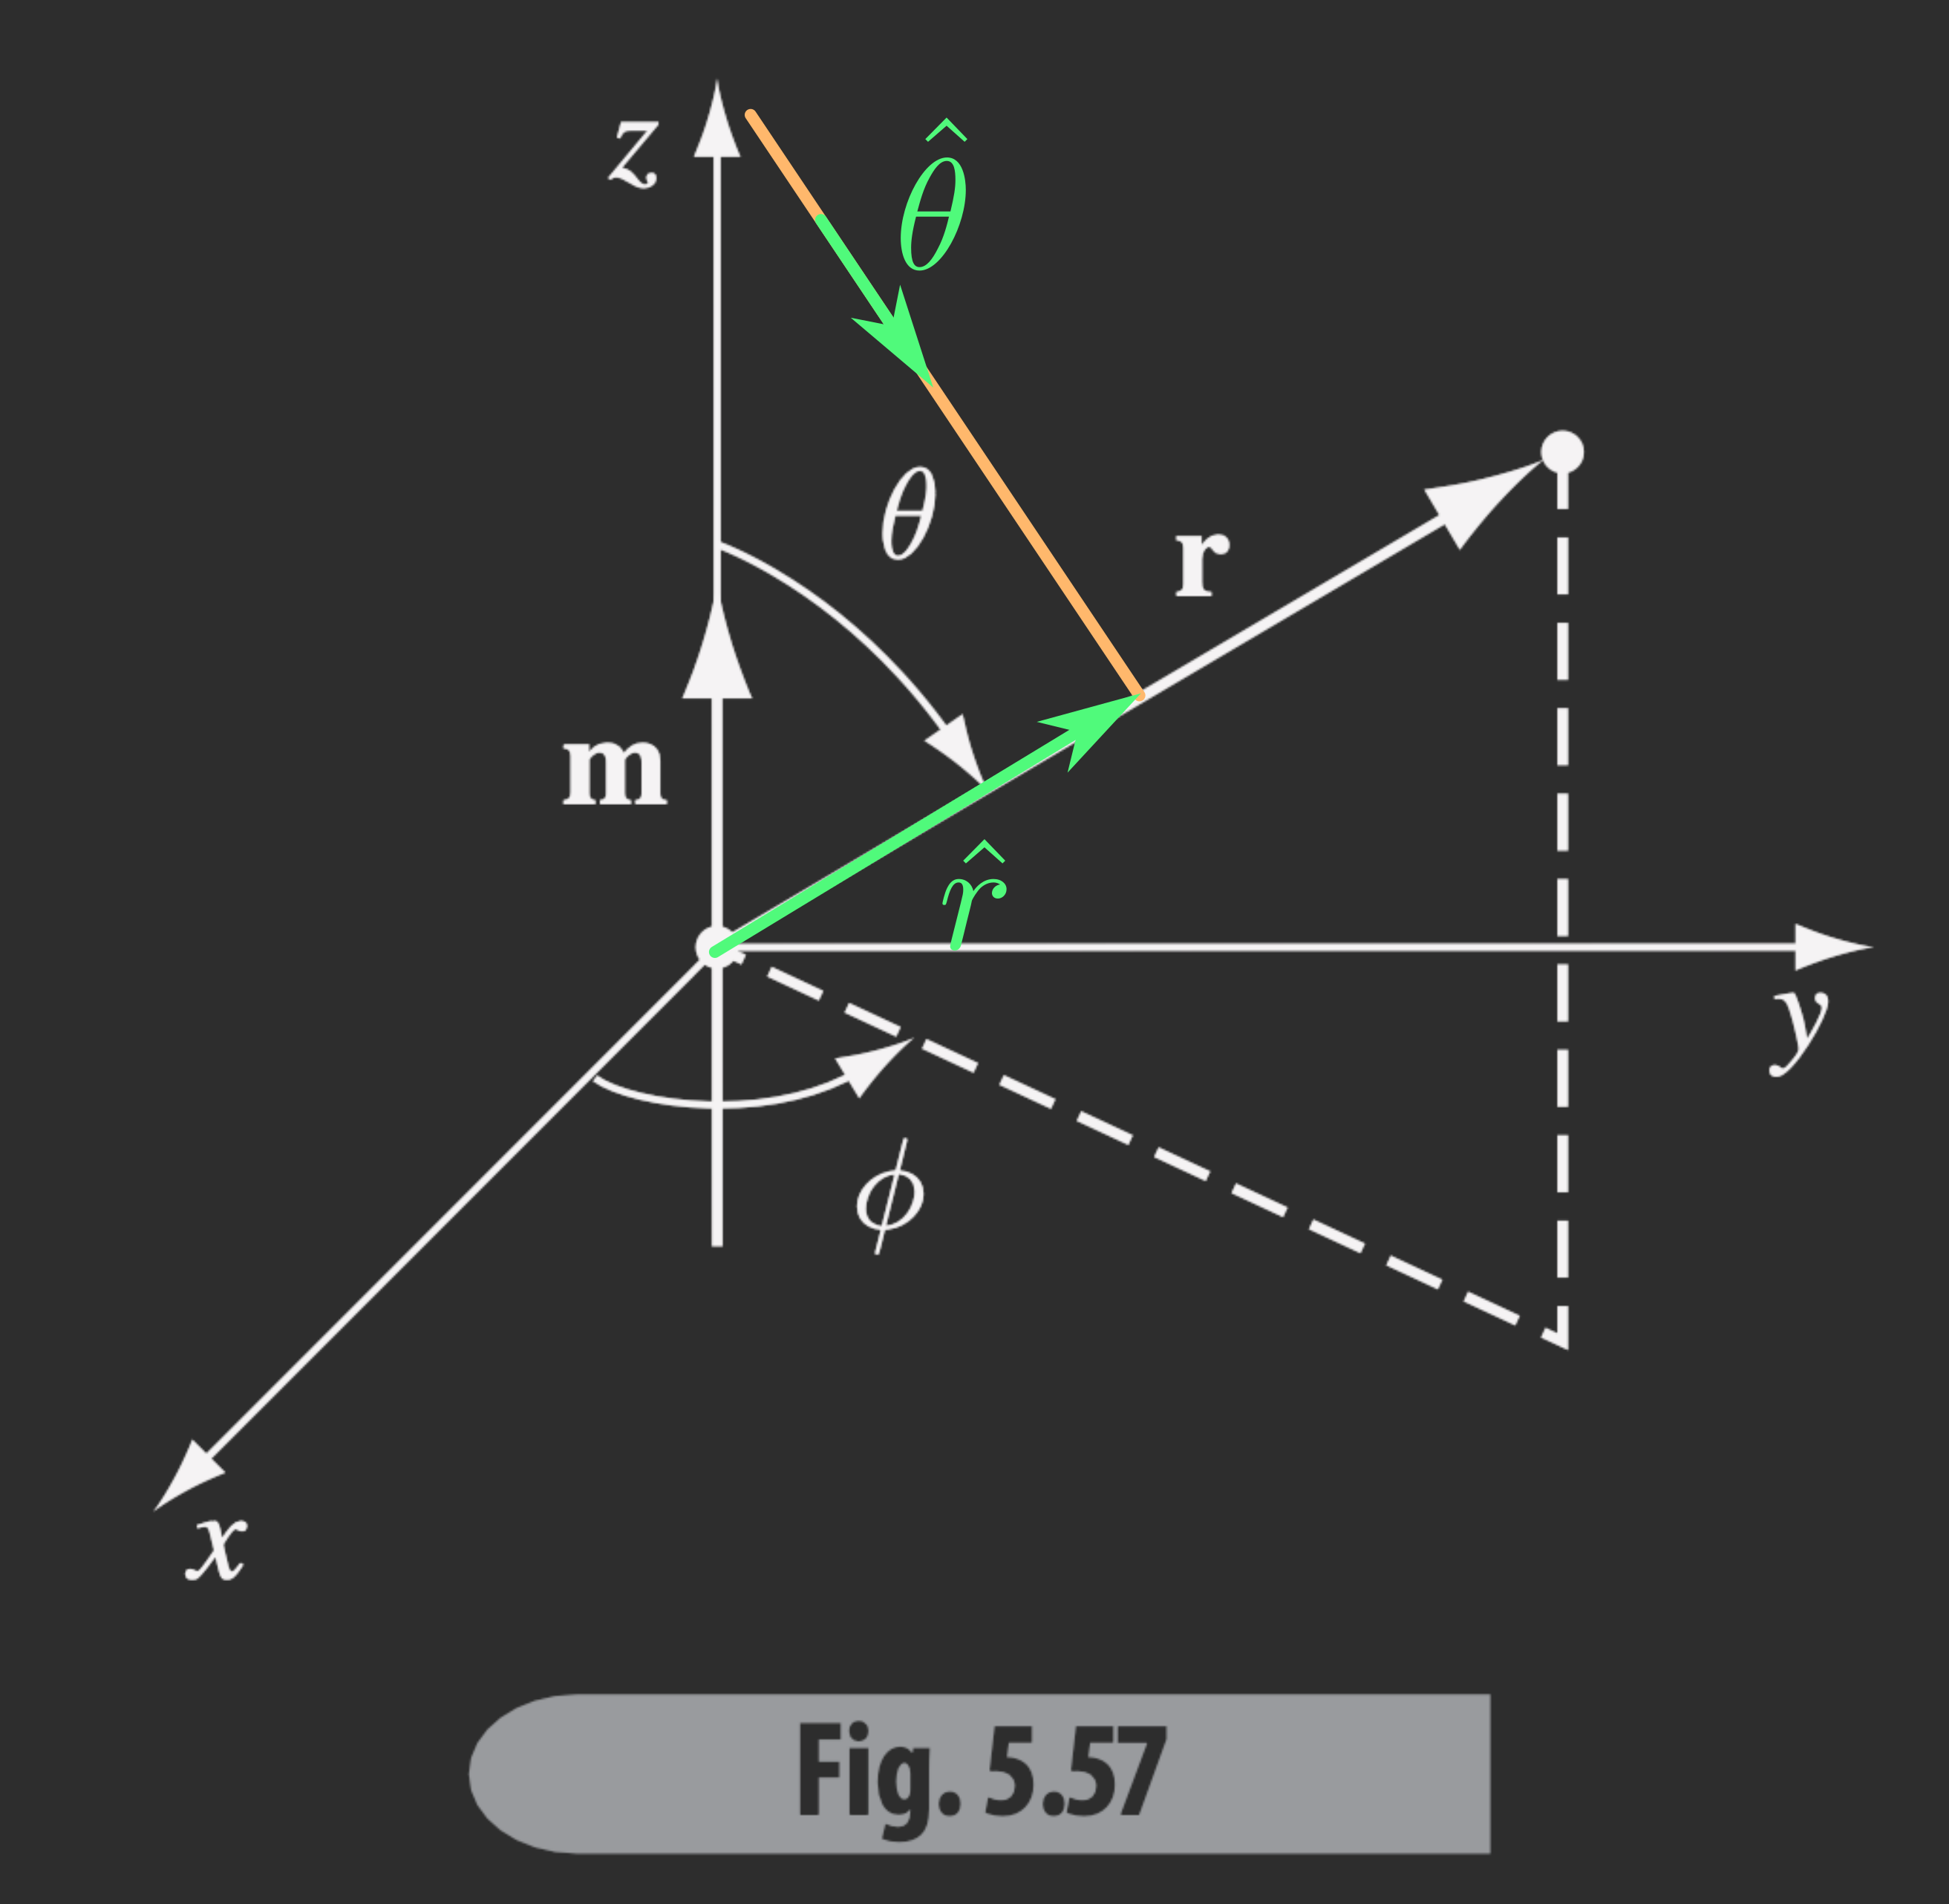
\includegraphics[width=0.5\textwidth]{hw9_1.png}
    \label{fig:5.32}
\end{figure*}
\paragraph{5.36} Show that thet magnetic dipole can be written in coordinate free form:
\begin{align*}\tag{5.89} \label{eq:5.89}
    \vb B_\text{dip} (\vb r) = \frac{\mu_0}{4\pi} \frac{1}{r^3} [
        3 (\vb m \cdot \vu r) \vu r - \vb m
    ] 
\end{align*}
From the Figure we can see that
\begin{align*}
    \vb m \cdot \vu r = m \cos\theta, \quad \vb m \cdot \vu*\theta = -m \sin\theta
\end{align*}
so
\begin{align*}
    \vb m = (\vb m \cdot \vu r) \vu r + (\vb m \cdot \vu*\theta) \vu*\theta = m \cos\theta \vu r - m \sin\theta \vu*\theta
\end{align*}
Therefore
\begin{align*}
    3(\vb m \cdot \vu r) \vu r - \vb m = 3m \cos\theta \vu r - (m \cos\theta \vu r - m \sin\theta \vu*\theta) = 2m \cos\theta \vu r + m \sin\theta \vu*\theta
\end{align*}
or from the textbook
\begin{align*} \tag{5.88}
    \vb B_\text{dip} (\vb r) = \frac{\mu_0 m}{4\pi r^3} \qt(
        2 \cos\theta \vu r + \sin\theta \vu*\theta
    )
\end{align*}

\newpage
\paragraph{5.39}
\begin{itemize}
    \item [(a)] A phonograph of radius $R$, surface charge $\sigma$ rotating at $\omega$, find its magnetic dipole moment:
    For a ring $\dd{r}$ using $v = \omega r$ and $I = \sigma v \dd{r}$ we have
    \begin{align*}
        m \equiv I \int \dd{\vb A}  = \sigma v (\pi r^2) \dd{r} = \pi \sigma \omega r^3 \dd{r}
    \end{align*}
    and integrating over the entire disk
    \begin{align*}
        m = \pi \sigma \omega \int_0^R r^3 \dd{r} = \frac{\pi \sigma \omega R^4}{4}
    \end{align*}
    \item [(b)] Find the magnetic dipole moment of a spinning spherical shell:
    For one ring of width $R \dd{\theta}$ around the sphere where $v = C / T$. For circumference $C = 2\pi R \sin\theta$ and time $T = 2\pi / \omega$,
    the current is
    \begin{align*}
        I = \sigma v (R \dd{\theta}) = \sigma \frac{2\pi R \sin\theta}{2\pi / \omega} \dd{\theta} = \sigma \omega R^2 \sin\theta \dd{\theta}
    \end{align*}
    Using the area around the ring $A = \pi (R\sin\theta)^2$, we can integrate over the entire sphere $\theta \in [0, \pi]$:
    \begin{align*}
        m = I A = \int \pi \sigma \omega R^2 \sin\theta (R\sin\theta)^2 \dd{\theta} &= \pi \sigma \omega R^4 \int_0^\pi \sin^3\theta \dd{\theta} \\
        = \pi \sigma \omega R^4 \int (\sin^2\theta) \sin\theta \dd{\theta} &= \pi \sigma \omega R^4 \int (1 - \cos^2\theta) \sin\theta \dd{\theta} \\
        \qusing \cos\theta = u &\implies -\sin\theta \dd{u} = \dd{\theta} \\
        = \pi\sigma \omega  R^4 \int (u^2 - 1) \dd{u} &= \pi\sigma \omega R^4 \qt[
            \frac{u^3}{3} - u
        ]_1^{-1} = \boxed{\frac{4}{3} \pi \sigma \omega  R^4}
    \end{align*}
    For $r > R$ the dipole term in the multipole expansion is
    \begin{align*}
        \vb A_\text{dip} = \frac{\mu_0}{4\pi} \frac{m \sin\theta}{r^2} \vu*\phi = \frac{\mu_0}{4\pi} \frac{4}{3} \pi \sigma \omega R^4 \frac{\sin\theta}{r^2} \vu*\phi = \boxed{\frac{1}{3r^2} \mu_0 \sigma \omega R^4 \sin\theta \vu*\phi}
    \end{align*}
    which is the same term from Problem 5.32 $\vb A = \vb A_\text{dip}$ thus a perfect dipole for points outside the sphere.
\end{itemize}

\end{document}